\documentclass[12pt]{book}
\usepackage{booktabs}
\usepackage[table]{xcolor}
\usepackage{tcolorbox}
\usepackage[T1]{fontenc}
\usepackage{wrapfig}
\usepackage{url}
\usepackage{dsfont}
\usepackage{enumitem}
\usepackage{array}
\usepackage{booktabs}
\usepackage{multirow}
\usepackage{mathtools, nccmath}
\usepackage[polish]{babel}
\usepackage[utf8]{inputenc}
\usepackage{lmodern}
\usepackage{pifont}
\usepackage{blkarray, bigstrut}
\usepackage{amsmath}
\usepackage{kbordermatrix}
\usepackage{cases}
\usepackage{graphicx}
\usepackage{cellspace}
\usepackage[T1]{fontenc}
\usepackage{amsthm}
\selectlanguage{polish}
\usepackage{amsmath}
\usepackage{graphicx}
\usepackage{float}
\usepackage{cite}
\usepackage[margin=2.5cm]{geometry}
\theoremstyle{plain}
\newtheorem{definicja}{Definicja}
\newtheorem{twr}{Twierdzenie}
\newtheorem{lem}[twr]{Lemat}
\newtheorem{mur}{Murphy}[section]
\newcolumntype{P}[1]{>{\centering\arraybackslash}p{#1}}
\newcommand\green{\cellcolor{green!10}}
\newcommand\cincludegraphics[2][]{\raisebox{-0.5\height}{\includegraphics[#1]{#2}}}
\newcommand\red{\cellcolor{red!20}}
\newcommand\blue{\cellcolor{blue!20}}
\newcommand{\R}{\mathbb{R}}
\newcommand*{\tabbox}[2][t]{%
	\vspace{0pt}\parbox[#1][3.7\baselineskip]{1cm}{\strut#2\strut}}
\newcommand\addtag{\refstepcounter{equation}
\renewcommand{\labelenumii}{\theenumii}
\renewcommand{\theenumii}{\theenumi.\arabic{enumii}.}
\tag{\theequation}}
\newcommand{\myref}[1]{(\ref{#1})} 
\newcommand{\specialcell}[2][c]{%
	\begin{tabular}[#1]{@{}c@{}}#2\end{tabular}}

\begin{document}
\title{Optymalizacja  systemu sygnalizacji świetlnej w 
oparciu o przepływowy model ruchu pojazdów.}
\author{Michał Lis}
\date{\today}
\maketitle
\tableofcontents
\chapter{Wprowadzenie}
Problem zatłoczonych ulic staje się coraz bardziej powszechny na całym świecie. W ogromnym tempie wzrasta ilość pojazdów na drogach.
%Problem zatłoczonych ulic staje się coraz bardziej powszechny na całym świecie, głównie ze względu na wzrost ekonomiczny. Według banku światowego w roku 1990 suma produktów krajowych brutto wszystkich państw świata wynosiła 22,6 biliona dolarów \cite{worldBank}. Najbardziej aktualne dane banku światowego dotyczą lat 2012-2017. W czasie ich trwania analogiczna wartość oscylowała wokół 75 bilionów dolarów. Nawet przy uwzględnieniu inflacji dolara, która od w okresie 1990 do 2015 wyniosła $80\%$ światowy produkt brutto jest obecnie prawie dwukrotnie większy w porównaniu do roku 1990. Bezpośrednim skutkiem ogólnoświatowego wzrostu stopy życiowej jest zwiększenie ilości samochodów na drogach.
Według danych firmy gromadzącej dane statystyczne \textit{Statista} liczba zarejestrowanych pojazdów na świecie w roku 2006 wynosiła 947 tysięcy \cite{liczbaPojazdowSwiat}. W 2015 roku na świecie jeździło już 1282 tysięcy pojazdów. Wzrost przez te 9 lat był niemalże liniowy. Co roku rejestrowano około 39,4 tysięcy nowych samochodów rocznie, co wyznacza stopę wzrostu liczby pojazdów na poziomie 3,7$\%$.
\begin{figure}[H]
  \centering
    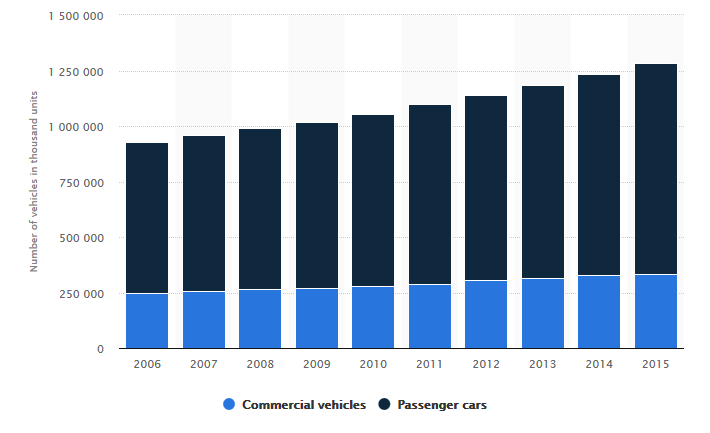
\includegraphics[width=14cm]{liczbaPojazdowSwiat}
 \caption{Liczba pojazdów na świecie}
 \label{fig:liczbaPojazdowSwiat}
\end{figure} \noindent
W Polsce wzrost ilości pojazdów w latach 2006 - 2015 był jeszcze większy \cite{liczbaPojazdowPolska}. W 2006 roku według GUS w Polsce było zarejestrowanych 13,4 miliona samochodów osobowych. W 2015 roku ich liczba wynosiła już 20,7 miliona, co oznacza 5 procentowy roczny wzrost.
Najbardziej zatłoczonym polskim miastem jest Łódź. Według rankingu firmy \textit{TomTom } Łódź zajmuje bardzo wysokie 5 miejsce na świecie i 1 w Europie pod względem zatłoczenia dróg \cite{rankingTomTom}. Oprócz Łodzi w pierwszej setce najbardziej zatłoczonych miast świata są inne polskie miasta: Lublin(34), Kraków(48), Warszawa(50), Wrocław(63), Poznań(69), Bydgoszcz(83). Problem całej Europy. Spośród 100 najbardziej zatłoczonych miast świata aż 45 znajduje się w Europie. W 2008 roku Unia Europejska oszacowała, iż koszty zatłoczenia dróg kształtują się na poziomie $0,9\%-1,5\%$ PKB unijnego \cite{ue2008}. Następny raport z 2017 roku może napawać optymizmem, gdyż przedstawione w nim wyliczenia określiły jedynie $0,77\%$ straty całkowitego PKB wspólnoty \cite{ue2017}. Ten sam raport ocenia koszty zatorów komunikacyjnych w Polsce na poziomie $1,2\%$ polskiego PKB.
Problemy zatorów komunikacyjnych w miastach są o tyle trudniejsze do rozwiązania niż poza miastem, ponieważ na terenach zurbanizowanych brakuje często miejsca na wybudowanie dróg o większej przepustowości. Rozwiązaniem może być wprowadzenie większej ilości sygnalizacji świetlnych. Istotną kwestią jest optymalizacja ustawień sygnalizacji świetlnej. Praca moja jest poświęcona temu problemowi. 
%W celu uzyskania danych potrzebnych do tego procesu rozstawiane są na drogach detektory ruchu. 
%\begin{figure}[H]
%  \centering
%    \includegraphics[width=14cm]{Detektor}
% \caption{System pętli do detekcji osi pojazdów zainstalowany na badawczym stanowisku pomiarowym na drodze DK81 będący w dyspozycji Katedry Metrologii i Elektroniki AGH.}
% \label{fig:Detektor}
%\end{figure} \noindent
%W miastach zachodnioeuropejskich rezultaty naprawdę widać dopiero po roku, gdy system zgromadzi już ogromną ilość danych - mówi Misiorny
%
%Czytaj więcej: https://dzienniklodzki.pl/masz-uwagi-do-sygnalizacji-swietlnej-w-lodzi-wyslij-email-do-zdit/ar/9253440
\chapter{Cel i zakres pracy}
Celem pracy jest stworzenie programu, który zoptymalizuje fazy sygnalizacji świetlnej, co przyczyni się do zwiększenia przepustowości sieci dróg.\\ Jako środowisko zostanie stworzony symulator ruchu drogowego. Symulacje ruchu będą w pełni zgodne z makroskopowym modelem ruchu. Sam makroskopowy model ruchu zostanie przedstawiony w rozdziale X. Jest to model ciągły. Pożądanym jest dyskretny model ruchu drogowego ze względu na łatwość implementacji komputerowej. Zostanie zatem przedstawiona w sekcji X.Y dyskretyzacja makroskopowego modelu ruchu. W rozdziale X zostanie zdefiniowany model sieci dróg. Początkowy model zaplanowano jako podstawowy z pominięciem większości aspektów. W każdej kolejnej sekcji model będzie stopniowo rozwijany. Sieci dróg zdefiniowane według końcowego modelu będą środowiskiem treningowym dla algorytmów uczenia maszynowego. Rozdział X opisuje uczenie ze wzmocnieniem - algorytm treningowy procesu optymalizacji sygnalizacji świetlnej. Rozdział X przedstawia cztery modele sieci dróg, dla których został stworzony program symulacyjny. Rozdział X opisuje optymalizację sygnalizacji świetlnej dla wspomnianych sieci dróg.


   
\chapter{Siatka czasowa i przestrzenna}
Dyskretny charakter modelu przedstawianego w pracy obliguje do określenia siatki czasowej i przestrzennej. Dla par czasu i miejsc należących do tych dwóch siatek będą określane zmienne stanu. \\ \\ \textbf{Siatka czasowa} jest zdefiniowana jako skończony ciąg liczb naturalnych:
\[(0,1,...,K). \addtag \]
Niech będzie ustalona droga $e$, która jest odcinkiem $[0,L_e]$. Droga zostaje podzielona na $L+1$ odcinków o równej długości $\Delta x=\frac{L_e}{L+1}$. \textbf{Siatka przestrzenna} drogi to ciąg odcinków:
\[(b_l)_{l=0}^{L}=[l\Delta x,(l+1)\Delta x]\]
\begin{figure}[H]
  \centering
    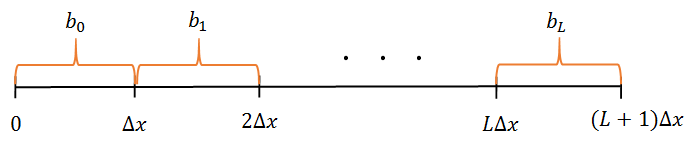
\includegraphics[width=14cm]{siatka_przestrzenna}
 \caption{Siatka przestrzenna}
 \label{fig:siatka_przestrzenna}
\end{figure}


\chapter{Makroskopowy model ruchu}
\section{Klasyfikacja modeli ruchu drogowego}
Modele ruchu drogowego mają na celu ukazanie rzeczywistego przepływu pojazdów w sposób czysto matematyczny. Ważnym kryterium doboru modelu jest przystępność jego implementacji informatycznej. Powszechnie klasyfikuje się 3 podejścia modelowe dla omawianego problemu \cite{CompareModels} - makroskopowy, mezoskopowy oraz mikroskopowy. Czasem \cite{multilevel} wyróżnia się także czwarte podejście - submikroskopowe. Jest to podział ze względu na poziom modelu. Najniższy poziom i najbardziej dokładny model gwarantuje podejście mikroskopowe. Rozważa ono pojazdy indywidualnie w czasoprzestrzeni. Przyspieszenie pojazdu jest wyliczane na podstawie dynamiki(prędkości, przyspieszenia) i pozycji pojazdu bezpośrednio przed nim. Model mezoskopowy zapewnia indywidualne rozróżnienie pojazdów, jednak ich zachowanie jest wyliczane na danych zagregowanych \cite{mesoscopic}. Przykładowo pojazdy są zgrupowane w grupę podróżującą z pewnego punktu startowego do celu. Inne modele \cite{mesoscopic2} mezoskopowe wyliczają dynamikę ruchu na podstawie aktualnego zatłoczenia drogi. Poziom mezoskopowy jest obliczeniowo bardziej opłacalny od mikroskopowego.
Wiele symulatorów stosujących model mezoskopowy oferuje symulację w czasie rzeczywistym dla sieci dróg całego miasta\cite{vu2017high}. Ideą modelu makroskopowego jest traktowanie ruchu ulicznego identycznie jak ruchu cieczy lub gazów. Po raz pierwszy w roku 1956 M. J. Lighthill i G. B. Whitham \cite{lwr} przedstawili pomysł przyrównania ruchu ulicznego na zatłoczonych drogach do przepływu wody w rzekach. Z tego powodu nie rozróżniamy w nim indywidualnie pojazdów, ani też nawet grupowo. Rozważamy natomiast gęstość ruchu w danym punkcie na drodze i czasie - czyli ilość pojazdów na danym odcinku drogi. Sposób w jaki poruszają się pojazdy jest wyliczany jedynie na podstawie gęstości ruchu. Jest to najmniej kosztowny obliczeniowo model. Właśnie w modelu makroskopowym zostało stworzone środowisko symulacyjne. Szczegóły modelu są przedstawione w następnym podrozdziale.

\section{Wstęp}
Istotą makroskopowego modelu ruchu jest pojęcie gęstości ruchu. Jest to zmienna stanowa określona dla każdego punktu drogi w czasie. Formalnie gęstość można rozumieć jako czynnik definiujący dynamikę ruchu. Im większa gęstość tym mniejsza prędkość ruchu. W niektórych artykułach gęstość ruchu \cite{helbing2001master} jest przedstawiona jako iloraz ilości pojazdów znajdujących się na pewnym odcinku i długości tego odcinka drogi. Nie są to jednak czysto matematyczne formalne definicje. W makroskopowym modelu nie rozróżniamy pojedynczych pojazdów, ani nawet grup, więc taka definicja gęstości ruchu może być odebrana jako nieścisła z ideą modelu. 
\section{Rozwój gęstości ruchu na drodze}
Makroskopowy model ruchu jest oparty o równanie różniczkowe (\ref{eq:main_diff_eq}) wraz z warunkiem początkowym (\ref{eq:p_init_eq}). Model makroskopowy traktuje ruch uliczny na drogach podobnie do przepływu wody w rzece[ref]. Gęstość ruchu można utożsamiać z polem powierzchni przekroju poprzecznego rzeki, co dla ustalonej szerokości rzeki - upraszcza się do wysokości wody w rzece. Istotną uwagą w tym miejscu jest zaznaczenie, iż rzeka zazwyczaj posiada pewien spadek, który zapewnia ruch cieczy ze źródła do ujścia. Ruch makroskopowy zdefiniowany przez równanie (\ref{eq:main_diff_eq}) z kolei odnosi się do rzeki która jest na całym swoim odcinku pozioma. W takim przypadku de facto nie ma zdefiniowanego zwrotu ruchu. \\Dla ustalonej drogi $e$ zmianę gęstości ruchu definiuje następujący układ równań:\\
\begin{numcases}{}
   p(x,0)=p_{0}(x) \label{eq:p_init_eq}
   \\
   \frac{\partial p(x,t)}{\partial t}+\frac{\partial f(p(x,t))}{\partial x}=0 \label{eq:main_diff_eq}
\end{numcases}
Gdzie $p(x,t)$ to gęstość ruchu w punkcie $x$ i czasie $t$. Wartość funkcji gęstości należy do przedziału $[0,p^{max}]$.\\
Równanie (\ref{eq:p_init_eq}) zakłada istnienie pewnej z góry nałożonej początkowej gęstości drogi $p_0(x)$.
Równianie (\ref{eq:main_diff_eq}) określa
wedle założeń modelu makroskopowego \cite{lwr} rozwój gęstości ruchu na drodze. Funkcja płynności ruchu $f$ powinna być wklęsła [ref]. W przedstawionym w tej pracy modelu funkcja ma następującą definicję:
\begin{numcases}{f(p)=}
   \lambda p & \text{dla } $p\in[0,p^{*}]$\\
   \lambda \cdot (2p^{*}-p) & \text{dla } $p\in(p^{*},p^{max}]$ 
\end{numcases}
Gdzie $\lambda$ jest stałym parametrem funkcji trójkątnej oraz $p^*=\frac{1}{2}p^{max}$.

\section{Dyskretyzacja makroskopowego modelu ruchu}
Niech będzie ustalona droga $e$ oraz jej siatka przestrzenna $b_l$. Celem jest przedstawienie wartości gęstości dla odcinków siatki przestrzennej w chwilach $k=0,1,...,K$.
Gęstość w odcinku $b_l$ i czasie $k$ jest zdefiniowana jako:
\[p_{l}^{k}=\int\limits_{{b_{l}}}{\frac{p(x,k)}{\Delta x}dx}. \addtag\]
Na podstawie (\ref{eq:main_diff_eq}) można wywnioskować, że:
\[\int\limits_{b_{l}} {p(x,k+1)- p(x,k)dx} +\int\limits_{k}^{k+1} f(b_{l+1},k)-f(b_{l},k))dk=0 \addtag \label{eq:calki-LWR} \]
Upraszczając otrzymujemy:
\[\Delta x(p_l^{k+1}-p_l^{k}) +\int\limits_{k}^{k+1} f(b_{l+1},k)-f(b_{l},k))dk=0=0 \addtag \]
Wartości gęstości zmieniają się w tylko w chwilach $k$. Wtedy wartości $f(b_{l+1},k)$ i $f(b_l,k)$ są stałe na całym przedziale całkowania $[k,k+1)$. Otrzymujemy równanie:
\[\Delta x(p_l^{k+1}-p_l^{k})  + (f(b_{l+1},k)-f(b_l,k))=0 \addtag \]
Rezultatem jest końcowy rekurencyjny wzór na gęstość ruchu:
\[p_l^{k+1}=p_l^{k}  -\frac{1}{\Delta x}  (f(b_{l+1},k)-f(b_l,k)) \addtag \]


\chapter{Model sieci dróg} \label{chapter:model_sieci_drog}
\section{Wstęp}
Ze względu na dużą złożoność końcowego modelu zostanie przedstawiony najpierw bardzo prosty, podstawowy model. W każdej kolejnej sekcji dodawane będą zmiany przybliżające do ostatecznej postaci. Jest to podejście pozwalające na proste przedstawienie modelu, który zawiera bardzo wiele aspektów m.in:
sygnalizacji świetlnej, wielu dróg, zatoru drogowego, źródła i ujścia ruchu. Zestawienie w jednej sekcji wszystkich tych kwestii byłoby bardzo przytłaczające.

\section{Wektor stanu drogi} \label{sec:wektor_stanu_drogi}
Wektor stanu jest strukturą przedstawiającą stan środowiska. Dla każdego odcinka drogi składuje on wartości zmiennych stanowych. Początkowo zmienna stanowa jest identyfikowana jako ilość pojazdów na danym odcinku drogi. 
\subsection{Przykład} \label{subsec:example-single-road}
Niech będzie dana droga z wydzielonymi czterema odcinkami. Przykładowy wektor stanu takiego środowiska to
\[\textbf{x(t)}=\begin{bmatrix}
2 \\ 4 \\ 3 \\ 0
\end{bmatrix} \addtag \]
Zawiera on w sobie następujące informacje dla chwili t:
\begin{itemize}
	\item Są 2 pojazdy na zerowym odcinku
	\item Są 4 pojazdy na pierwszym odcinku
	\item Są 3 pojazdy na drugim odcinku
	\item Nie ma żadnego pojazdu na trzecim odcinku
\end{itemize}

\begin{figure}[H]
	\centering
	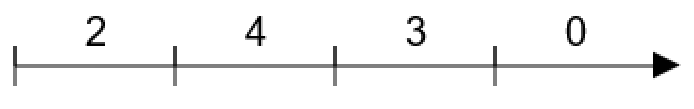
\includegraphics[width=14cm]{images/1_droga_4_odcinki}
	\caption{Droga z ilością pojazdów na poszczególnych odcinkach}
	\label{fig:single_road}
\end{figure}
\section{Rozwój wektora stanu jednej drogi}
Początkowy model przepływu pojazdów zakłada, iż wszystkie pojazdy w chwili t+1 są o jeden odcinek dalej w swojej podróży niż w momencie $t$. Założone jest, iż żadne nowe pojazdy nie pojawiają się w sieci dróg. Ujście pojazdów znajduje się na końcu ostatniego odcinka. Wszystkie pojazdy będące w chwili $t$ na ostatnim odcinku w chwili $t+1$ opuszczają układ. Formalnym wzorem definiującym rozwój wektora stanu jest:
\[\textbf{x(t+1)}=\textbf{Ax(t)} \addtag \label{eq:single_road} \]
Gdzie $\textbf{A}$ jest macierzą systemu. Definiuje ona sposób przepływu pojazdów. $\textbf{A}$ jest rzadką, kwadratową macierzą o wartościach równych 1 jedynie bezpośrednio 1 wiersz pod główną przekątną macierzy. Takie wartości gwarantują przepływ pojazdów o jeden odcinek w jednym interwale czasowym.
\subsection{Przykład}
Dla przykładu przedstawionego w (\ref{subsec:example-single-road}) zostanie przedstawiony rozwój wektora stanu. Niech zatem
\def \xZero {\begin{bmatrix}
	2 \\ 4 \\ 3 \\ 0
	\end{bmatrix}}
\[\textbf{x(0)}=\xZero \addtag \]
Macierzą systemu jest:
\def \A {\begin{bmatrix}
		0 & 0 & 0 & 0 \\
		1 & 0 & 0 & 0 \\
		0 & 1 & 0 & 0 \\
		0 & 0 & 1 & 0 \\
\end{bmatrix}}

\[
\textbf{A}=\A \addtag
\]
Wedle wzoru (\ref{eq:single_road}) wyliczone zostają kolejne wartości wektora stanu.
\def \xI {\begin{bmatrix}
		0 \\ 2 \\ 4 \\ 3
\end{bmatrix}}
\[
\textbf{x(1)}=\textbf{Ax(0)}=\A \xZero = \xI \addtag
\]
\def \xII {\begin{bmatrix}
		0 \\ 0 \\ 2 \\ 4
\end{bmatrix}}
\[
\textbf{x(2)}=\textbf{Ax(1)}=\A \xI = \xII \addtag
\]
\def \xIII {\begin{bmatrix}
		0 \\ 0 \\ 0 \\ 2
\end{bmatrix}}
\[
\textbf{x(3)}=\textbf{Ax(2)}=\A \xII = \xIII \addtag
\]
\def \xIV {\begin{bmatrix}
		0 \\ 0 \\ 0 \\ 0
\end{bmatrix}}
\[
\textbf{x(4)}=\textbf{Ax(3)}=\A \xIII = \xIV \addtag
\]

\section {Wektor stanu sieci dróg}
W rozdziale (\ref{sec:wektor_stanu_drogi}) przedstawiony został wektor stanu dla pojedynczej drogi. W tym rozdziale zostanie sformułowany wektor stanu dla bardziej ogólnego przypadku - sieci dróg. Sposób przedstawienia wartości stanuch jednak jest bardzo podobny. Każda z dróg $e_1,...,e_n$ ma $k$ wydzielonych odcinków oznaczanych jako $b_1,...,b_{nk}$. Dla każdego z odcinków definiowana jest wartość stanowa.

\subsection{Przykład} \label{subsec:wektor_stanu_siec_przyklad}
Niech będzie dana sieć składająca się z trzech dróg. Dla każdej drogi zostaną wydzielone 2 odcinki. W sumie środowisko posiada 6 odcinków. Odcinki są ponumerowane od 0 co przedstawia poniższy rysunek.
	\begin{figure}[H]
	\centering
	
\includegraphics[width=10cm]{images/env_11}
	\label{fig:env_11}
	\caption{Numeracja odcinków środowiska}
\end{figure}

Niech przykładowym wektorem stanu będzie:
\def \xzero {\begin{bmatrix}
		8 \\ 4 \\ 3 \\ 0 \\ 1 \\ 5
\end{bmatrix}}

\[\textbf{x(t)}=\xzero \addtag \]
Zawiera on w sobie informacje dotyczące ilości pojazdów na poszczególnych odcinkach w chwili t. Poniższy obraz przedstawia ilości pojazdów na poszczególnych odcinkach dla stanu zadanego przez wektor $\textbf{x(t)}$
\begin{figure}[H]
	\centering
	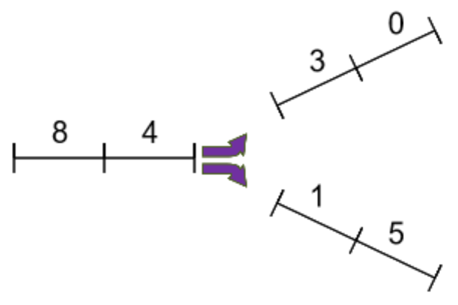
\includegraphics[width=10cm]{images/env_11_843015}
	\caption{Sieć dróg z ilościami pojazdów na poszczególnych odcinkach}
	\label{fig:3_single_road}
\end{figure}

\section{Rozwój wektora stanu sieci dróg}
Przepływ pojazdów niezmiennie jest oparty o założenie, iż w trakcie trwania jednego interwału czasowego pojazdy pokonują 1 odcinek drogi. Nie pojawiają się nowe pojazdy w trakcie trwania symulacji, a ujścia ruchu znajdują się na końcu odcinków 3 i 5.
%Równaniem systemu pozostaje $\textbf{x(t+1)=Ax(t)}$, gdyż do układu nie wpływają nowe pojazdy.\\ \\
Macierz systemu $\textbf{A}$ powinna uwzględnić przepływy pojazdów na skrzyżowaniach. Do tej pory wszystkie pojazdy poruszały się do przodu. W przypadku sieci dróg trzeba uwzględnić przypadek skrzyżowania, gdzie pojazdy mogą obrać różne kierunki ruchu.
%W tym momencie należy przedstawić następującą definicję macierzy $\textbf{A}$:\\
%Wartości macierzy \textbf{A} określają jaka część pojazdów z odcinka zadanego przez indeks kolumny przejeżdża do odcinka zadanego przez indeks wiersza. 
Zdefiniowana zostanie zatem macierz $ \textbf{P} $ prawdopodobieństwa manerwów. Jest to niezmienna w czasie rzadka macierz. Wartości macierzy $ \textbf{P} $ w kolumnie i oraz wierszu j to prawdopodobieństwo przejazdu pojazdu będącego na odcinku i do odcinka j.


\subsection{Przykład}
Rozważone zostanie środowisko (\ref{subsec:wektor_stanu_siec_przyklad}) z dodatkowym założeniem, że 75 procent pojazdów ma zamiar skręcić w prawo. Pozostałe 25 procent wybiera skręt w lewo. 
Srodowisko przedstawiają poniższe obrazki.

\begin{tabular}{| c  | Sc |}
	\hline
	Numeracja odcinków   & Ilości pojazdów \\
	\hline
	\cincludegraphics[width=7cm]{images/env_11}  & \cincludegraphics[width=7cm]{images/env_11_843015_procenty} \\
	\hline 
\end{tabular}

Taki sposób przepływu definiuje rzadką macierz prawdopodobieństwa $ \textbf{P} $ o wymiarach 6 na 6.
\begin{itemize}
	\item $\textbf{P}[1,2]=0.25$ wyznacza manewr skrętu w lewo
	\item $\textbf{P}[1,4]=0.75$ wyznacza manewr skrętu w prawo
	\item $\textbf{P}[0,1]=1 \;\; \textbf{P}[2,3]=1 \;\; \textbf{P}[4,5]=1$ co wynika z przepływu pojazdów pomiędzy sekcjami na jednej drodze
	\item Pozostałe wartości macierzy $\textbf{P}$ to zera.
\end{itemize}

\def \P {\begin{bmatrix}
		0 & 0 & 0 & 0 & 0 & 0 \\
		1 & 0 & 0 & 0 & 0 & 0 \\
		0 & 0.25 & 0 & 0 & 0 & 0 \\
		0 & 0 & 1 & 0 & 0 & 0 \\
		0 & 0.75 & 0 & 0 & 0 & 0 \\
		0 & 0 & 0 & 0 & 1 & 0 
\end{bmatrix}}
\[P=\P\]





\def \A{
\begin{bmatrix}
	0 & 0    & 0 & 0 & 0 & 0 \\
	1 & 0    & 0 & 0 & 0 & 0 \\
	0 & 0.25 & 0 & 0 & 0 & 0 \\
	0 & 0    & 1 & 0 & 0 & 0 \\
	0 & 0.75 & 0 & 0 & 0 & 0 \\
	0 & 0    & 0 & 0 & 1 & 0 
\end{bmatrix}
}
\begin{flushleft}
W sytuacji gdy nie ma uwzględnionej sygnalizacji świetlnej oraz pojęcia zatoru macierz systemu jest macierzą prawdopodobieństwa, czyli $A=P$. \linebreak Wartości wektora stanu zmieniają się zgodnie równaniem stanu $\textbf{x(t)}=\textbf{Ax(t-1)}$. Poniżej zapisane są obliczenia.
\end{flushleft}

\def \xI{\begin{bmatrix}
		0 \\ 8 \\ 1 \\ 3 \\ 3 \\ 1
\end{bmatrix}}
\def \xII{\begin{bmatrix}
		0 \\ 0 \\ 2 \\ 1 \\ 6 \\ 3
\end{bmatrix}}
\def \xIII{\begin{bmatrix}
		0 \\ 0 \\ 0 \\ 6 \\ 0 \\ 2
\end{bmatrix}}
\begin{tabular}{| c | c | Sc |}
	\hline
	t   & Równanie stanu & Podgląd środowiska \\
	\hline
	0 & 
	$ \textbf{x(0)} = \xzero$  & \cincludegraphics[width=7cm]{images/env_11_843015_procenty} \\
	\hline 
	1 & $\textbf{x(1)}=\textbf{Ax(0)}=\A \xzero = \xI$  & \cincludegraphics[width=7cm]{images/env_11_081331_procenty} \\
	\hline 
	2 & $\textbf{x(2)}=\textbf{Ax(1)}=\A \xI = \xII$  & \cincludegraphics[width=7cm]{images/env_11_002163_procenty} \\
	\hline 
	3 &	$\textbf{x(3)}=\textbf{Ax(2)}=\A \xII = \xIII$ & \cincludegraphics[width=7cm]{images/env_11_000602_procenty} \\
\hline 
\end{tabular}


\newpage
\section{Wprowadzenie sygnalizacji świetlnej}
Kolejnym etapem rozwoju modelu jest wprowadzenie sygnalizacji świetlnej. Warto zauważyć, że do tej pory rozważane układy były pozbawione jakiegokolwiek sterowania, czego bezpośrednim skutkiem była niezmienność macierzy $\textbf{A}$ w czasie. 
Niech wektor $ [i,j] $ będzie manewrem polegającym na bezpośrednim przejeździe z odcinka $ i $ na odcinek $ j $. Zostanie teraz zdefiniowana macierz sygnalizacji świetlnej $\textbf{S}$. Określa ona wykonalność dowolnego manewru.

\begin{numcases}{S_{ij}=}
1 & dla manewru zezwolonego przez zielone światło \label{eq:allowed_by_light} \\
1 & dla manewru nie wymagającego sygnalizacji świetlnej \label{eq:manewr_existing} \\
0 & dla manewru wstrzymanego przez czerwone światło \label{eq:stopped_by_light} \\
0 & dla niemożliwego manewru \label{eq:manewr_not_existing}
\end{numcases}
Sygnalizacja świetlna zawsze posiada pewną fazę, która określa dozwolone \myref{eq:allowed_by_light} oraz niedozwolone \myref{eq:stopped_by_light} manewry. Fazy świetlne będą oczywiście zmieniane w trakcie symulacji zatem macierz $\textbf{S}$ też jest zmienna w czasie. Wartości macierzy $\textbf{S}$ obejmujące przypadki \ref{eq:manewr_not_existing} oraz \ref{eq:manewr_existing} są z kolei niezmienne dla ustalonego środowiska.
\subsection{Przykład macierzy sygnalizacji świetlnej} \label{subsec:macierz_sygnalizacji}
Rozważone będzie znane z poprzednich przykładów skrzyżowanie - tym razem mające sygnalizację świetlną z aktywną fazą zezwalającą na manewr [1,2]. Ta sama faza zabrania przejazdu z 1 odcinka do 4. 

\begin{tabular}{| Sc  | Sc |}
	\hline
	Numeracja odcinków   & Ilości pojazdów \\
	\hline
	\cincludegraphics[width=7cm]{images/env_11_faza_0_procenty}  & \cincludegraphics[width=7cm]{images/env_11_lights_0_943015_procenty} \\
	\hline 
\end{tabular}

Poszczególne manewry są następujące:
\begin{itemize}
	\item \myref{eq:allowed_by_light} - Manewrem zezwolonym przez zielone światło  dla fazy $ 0 $ jest $ [1,2] $.
	\item \myref{eq:manewr_existing} - Prawidłowym manewrem bez sygnalizacji świetlnej są manewry $ [0,1] $, $ [2,3] $, $ [4,5] $.
	\item \myref{eq:stopped_by_light} - Dla fazy świetlnej $ 0 $ manewrem zatrzymanym przez czerwone światło  jest $ [1,4] $.
	\item \myref{eq:manewr_not_existing} - Pozostałe manewry są niemożliwe. Przykładem niech będzie $ [0,2] $, gdyż nie ma możliwości bezpośredniego przejazdu z odcinka $ 0 $ do $ 2 $. Teoretycznie możliwy mógłby się wydawać manewr [1,1] jednak jest on uznany za niemożliwy.
\end{itemize}
Macierz sygnalizacji świetlnej dla tego przykładu jest następująca:
\def \S{\begin{bmatrix}
		0 & 0 & 0 & 0 & 0 & 0 \\
		1 & 0 & 0 & 0 & 0 & 0 \\
		0 & 0 & 0 & 0 & 0 & 0 \\
		0 & 0 & 1 & 0 & 0 & 0 \\
		0 & 0 & 0 & 0 & 0 & 0 \\
		0 & 0 & 0 & 0 & 1 & 0 \\
\end{bmatrix}}
\[\textbf{S}=\S\]


\subsection{Macierz systemu uwzględniająca sygnalizację świetlną}
Mając zdefiniowaną zarówno macierz prawdopodobieństwa przejazdów $\textbf{P}$ jak i macierz sygnalizacji świetlnej $ \textbf{S} $ można ustalić macierz systemu $\textbf{A}$ uwzględniającą już sygnalizacje świetlne. Niech $Q$ będzie zbiorem odcinków, które znajdują się bezpośrednio przed ujściem ruchu. Wtedy macierz systemu zdefiniowana jest jako: 
\begin{numcases}{A[i,j]=}
0 & dla $S[i,j]=0 \vee i \in {Q}$ \\
P[i,j] & dla $ S[i,j]=1$ \\
1-\delta(i) & dla $i=j \wedge  i \not\in {Q}$
\end{numcases}
Równanie systemu jest następujące:
\[\textbf{x(t+1)}=\textbf{A(t)x(t)} \addtag \]
Macierz systemu jest teraz zmienna w czasie, zatem w miejse $\textbf{A}$ dotychczasowego równania pojawiło się $\textbf{A(t)}$. \\ \\
\subsection{Przykład rozwoju wektora stanowego}
Niech dla chwili t=0 będzie dany układ z przykładu \myref{subsec:macierz_sygnalizacji}. W chwili t=2 zostanie zmieniona faza świetlna. Od tego momentu obydwa manewry na skrzyżowaniu są dozwolone.  W chwili t=3 wartości stanowe nie są całkowite, co nie przeszkadza modelowi matematycznemu. Wartości stanowe były identyfikowane do tej pory jako ilość pojazdów na odcinku i dalej jest to dobra interpretacja o ile przyjmiemy, że pojazdy są możliwe do podzielenia na części. Rozwój wektora stanu został przedstawiony w poniższej tabeli.

\def \xzero{\begin{bmatrix}
		9 \\ 4 \\ 3 \\ 0 \\ 1 \\ 5
\end{bmatrix}}
\def \xI{\begin{bmatrix}
		0 \\ 12 \\ 1 \\ 3 \\ 0 \\ 1
\end{bmatrix}}
\def \xII{\begin{bmatrix}
		0 \\ 9 \\ 3 \\ 1 \\ 0 \\ 0
\end{bmatrix}}
\def \xIII{\begin{bmatrix}
		0 \\ 0 \\ 2 \frac{1}{4} \\ 3 \\ 7 \frac{3}{4} \\ 0
\end{bmatrix}}

\def \AZero{
	\begin{bmatrix}
		0 & 0            & 0 & 0 & 0 & 0 \\
		1 & \frac{3}{4}  & 0 & 0 & 0 & 0 \\
		0 & \frac{1}{4}  & 0 & 0 & 0 & 0 \\
		0 & 0            & 1 & 0 & 0 & 0 & \\
		0 & 0            & 0 & 0 & 0 & 0 \\
		0 & 0            & 0 & 0 & 1 & 0 \\
	\end{bmatrix}	
}

\def \AI{
	\begin{bmatrix}
	0 & 0            & 0 & 0 & 0 & 0 \\
	1 & \frac{3}{4}  & 0 & 0 & 0 & 0 \\
	0 & \frac{1}{4}  & 0 & 0 & 0 & 0 \\
	0 & 0            & 1 & 0 & 0 & 0 & \\
	0 & 0            & 0 & 0 & 0 & 0 \\
	0 & 0            & 0 & 0 & 1 & 0 \\
\end{bmatrix}	
}
\def \AII{
	\begin{bmatrix}
	0 & 0            & 0 & 0 & 0 & 0 \\
	1 & 0            & 0 & 0 & 0 & 0 \\
	0 & \frac{1}{4}  & 0 & 0 & 0 & 0 \\
	0 & 0            & 1 & 0 & 0 & 0 & \\
	0 & \frac{3}{4}  & 0 & 0 & 0 & 0 \\
	0 & 0            & 0 & 0 & 1 & 0 \\
\end{bmatrix}
}

\centerline{
\begin{tabular}{| c | c | Sc |}
	\hline
	t   & Równanie stanu & Podgląd środowiska \\
	\hline
	0 &
	$ \textbf{x(0)} = \xzero$  & \cincludegraphics[width=7cm]{images/env_11_lights_0_943015_procenty} \\
	\hline 
	1 & $\textbf{x(1)}=\textbf{A(0)x(0)}=\AZero \xzero = \xI$  & \cincludegraphics[width=7cm]{images/env_11_lights_0_0121301_procenty} \\
	\hline 
	2 & $\textbf{x(2)}=\textbf{A(1)x(1)}=\AI \xI = \xII$  & \cincludegraphics[width=7cm]{images/env_11_lights_01_093100_procenty} \\
	\hline 
	3 &	$\textbf{x(3)}=\textbf{A(2)x(2)}=\AII \xII = \xIII$ & \cincludegraphics[width=7cm]{images/env_11_lights_koncowe_procenty} \\
	\hline 
\end{tabular}
}




\section{Wprowadzenie źródeł ruchu }
Wszystkie poprzednie przykłady układów ruchu drogowego szybko kończyły się stanem w którym nie było już żadnych pojazdów na drogach. W tej sekcji zostanie przedstawiony sposób napływania nowych pojazdów do układu. 
Wprowadzony zostanie wektor źródłą $\textbf{u(t)}$ definiujący pojazdy pojawiające się w układzie. Jest on zmienny w czasie, a jego wartości określają ile pojazdów pojawia się w następnej chwili w poszczególnych odcinkach układu.
Równanie systemu uwzględniające zródła ruchu to:
\[\textbf{x(t)}=\textbf{A(t-1)x(t-1)} + \textbf{u(t-1)} \label{eq:stan_u}   \addtag{}\]
\subsection{Przykład}
Rozważony zostanie prosty przykład, który nie uwzględnia wcześniej wprowadzonych pojęć sygnalizacji świetlnej oraz zatoru. Przedstawione zostanie środowisko składające się z dwóch dróg, które nie są ze sobą w żaden sposób połączony.
\begin{figure}[H]
	\centering
	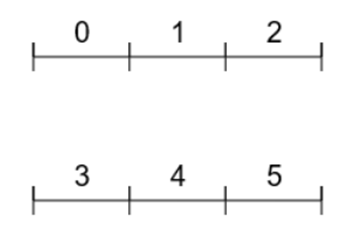
\includegraphics[width=8cm]{images/env_12}
	\label{fig:env_12}
	\caption{Numeracja odcinków środowiska}
\end{figure} \noindent
Pojazdy wzdłóż dróg kończąc swój bieg po przejechaniu przez odcinki 5 i 2 co przedstawia macierz systemu $A$:
\def \A{\begin{bmatrix}
0 & 0 & 0 & 0 & 0 & 0 \\
1 & 0 & 0 & 0 & 0 & 0 \\
0 & 1 & 0 & 0 & 0 & 0 \\
0 & 0 & 0 & 0 & 0 & 0 \\
0 & 0 & 0 & 1 & 0 & 0 \\
0 & 0 & 0 & 0 & 1 & 0
\end{bmatrix}}
\[A=\A \]
Pragnąc by do odcinków 0 i 3  napływało odpowiednio po 4, 8, 20 oraz 3, 7, 5 pojazdów należy zdefiniować ciąg wektorów $\textbf{u(t)}$ w sposób przedstawiony w poniższej tabeli.

\def \xzero{\begin{bmatrix}
		0 \\ 8 \\ 1 \\ 3 \\ 3 \\ 1
\end{bmatrix}}
\def \xI{\begin{bmatrix}
		4 \\ 0 \\ 8 \\ 3 \\ 3 \\ 3
\end{bmatrix}}
\def \xII{\begin{bmatrix}
		8 \\ 4 \\ 0 \\ 7 \\ 3 \\ 3
\end{bmatrix}}
\def \xIII{\begin{bmatrix}
		20 \\ 8 \\ 4 \\ 5 \\ 7 \\ 3
\end{bmatrix}}
\def \uZero{\begin{bmatrix}
		4 \\ 0 \\ 0 \\ 3 \\ 0 \\ 0
\end{bmatrix}}
\def \uI{\begin{bmatrix}
		8 \\ 0 \\ 0 \\ 7 \\ 0 \\ 0
\end{bmatrix}}
\def \uII{\begin{bmatrix}
		20 \\ 0 \\ 0 \\ 5 \\ 0 \\ 0
\end{bmatrix}}

\centerline{
\begin{tabular}{| c | c | Sc | c |}
	\hline
	t   & Równanie stanu & Podgląd środowiska & $ \textbf{u(t)} $ \\
	\hline
	0 & 
	$ \textbf{x(0)} = \xzero$  & \cincludegraphics[width=5cm]{images/env_12_t0} & $\uZero$ \\
	\hline 
	1 & $\textbf{x(1)}=\textbf{Ax(0)}+\textbf{u(0)}=\A \xzero + \uZero = \xI$  & \cincludegraphics[width=5cm]{images/env_12_t1} & $\uI $ \\
	\hline 
	2 & $\textbf{x(2)}=\textbf{Ax(1)}+\textbf{u(1)}=\A \xI + \uI = \xII$  & \cincludegraphics[width=5cm]{images/env_12_t2} & $\uII $ \\
	\hline 
	3 &	$\textbf{x(3)}=\textbf{Ax(2)}+\textbf{u(2)}=\A \xII + \uII = \xIII$ & \cincludegraphics[width=5cm]{images/env_12_t3} & \\
	\hline 
\end{tabular}
}
\subsection{Zatory drogowe}
Dotychczasowe przedstawienie macierzy systemu $ \textbf{A} $ nie zawiera w sobie jeszcze pojęcia zotoru drogowego. W jednym interwale czasowym moze przejechac przez odcinek astronomiczna wrecz liczba pojazdów. Wprowadzona zostanie zatem funkcja zatoru ograniczająca przejazdy w przypadku zbyt dużej liczby pojazdów. Dziedziną funkcji zatoru $ f $ jest zbiór wszystkich manewrów $ [i,j] $, takich że $ i \neq j $. Funkcja zatoru jest jednak zależna także od wartości stanowych wektora $\textbf{x}$, a przede wszystkim od ilości pojazdów na odcinkach $i$ oraz $j$ czyli $x[i],x[j]$. Wartości funkcji $f$ należą do przedziału $[0,1]$.
Macierz stanowa $\textbf{A}$ z uwzględnieniem zatorów dla układu z $ n $ odcinkami przedstawia się następująco:

\def \Af {\begin{bmatrix}
		1-\delta(0) & f(1,0) & ... & f(n,0) \\
		f(0,1) &1-\delta(1)& ... & f(n,1) \\
		f(0,2) &f(1,2)& ... & f(n,2) \\
		...   &...& ... & ... \\
		f(0,n) &f(1,n)& ... & 1-\delta(n)
\end{bmatrix}}

\[\textbf{A}=\Af \addtag \label{eq_A_z_korkiem} \]
Gdzie $\delta$ to suma wszystkich wartości danej kolumny z wyłączeniem tych na głównej przekątnej. W przypadku odcinków zakończonych ujściem, aby wyzerować wartości $\delta$ przyjmuje wartość 1. Formalnie $\delta$ to:
\begin{numcases}{\delta(i)=}
\sum_{j\in{\{0,...,n\}},j!=i} f(i,j) & dla odcinka $i$ nie zakończonego ujściem \\
1 & dla odcinka $i$ zakończonego ujściem
\end{numcases}

\subsection{Przykład zatoru na pojedynczej drodze} \label{subsec:zator_f10}
Rozważmy poniższe środowisko składające się z drogi posiadającej 4 odcinki.
\begin{figure}[H]
	\centering
	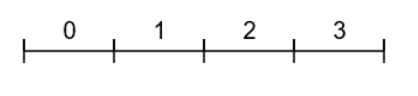
\includegraphics[width=14cm]{images/env_13}
	\caption{Droga z numeracją odcinków}
	\label{fig:env_13}
\end{figure}
Należy skonstruować pewną funkcję zatoru. Niech jej celem będzie, aby przez jeden interwał czasowy maksymalnie 10 pojazdów przejeżdżało przez odcinek drogi. Następująca funkcja gwarantuje takie zachowanie:

\begin{numcases}{f(i,j)=}
\textbf{P}[i,j] & dla $ j=i+1 \wedge x[i]<10$ - przejazd bez zatoru \label{eq:manewr_bez_zatoru_f10} \\
\frac{10}{x[i]} & dla $ j=i+1  \wedge x[i] \geq 10$ - przejazd z zatorem \label{eq:manewr_zator_f10} \\
0 & dla pozostałych przypadków - niemożliwe manewry
\end{numcases} \noindent
 Macierze stanowe zostały wyliczone na podstawie wzoru \ref{eq_A_z_korkiem}. W tym przypadku jest to:
\def \A {\begin{bmatrix}
		1-\delta(0) & f(1,0) &   f(2,0) & f(3,0) & \\
		f(0,1) & 1-\delta(1) &   f(2,1) & f(3,1) & \\
		f(0,2) & f(1,2) &   1-\delta(2) & f(3,2) & \\
		f(0,3) & f(1,3) &   f(2,3) & 1-\delta(3) & \\
\end{bmatrix}}
\[A=\A \label{eq:A_1droga_korek}\]

Funkcja $\delta$ dla tego środowiska to:
\begin{numcases}{\delta(i)=}
\sum_{j\in{\{0,1,2,3\}},j!=i} f(i,j) & dla $i \in {0,1,2}$ \\
1 & dla $i = 3 $
\end{numcases}

\def \xzero {\begin{bmatrix}
		17 \\ 2 \\ 11 \\ 4
\end{bmatrix}}

\def \xI {\begin{bmatrix}
		7 \\ 10 \\ 3 \\ 10
\end{bmatrix}}

\def \xII {\begin{bmatrix}
		0 \\ 6 \\ 10 \\ 3
\end{bmatrix}}

\def \Azero {\begin{bmatrix}
		\frac{7}{17} & 0 & 0 & 0  \\
		\frac{10}{17} & 0 & 0 & 0  \\
		0 & 1 & \frac{1}{11} & 0  \\
		0 & 0 & \frac{10}{11} & 0  \\
\end{bmatrix}}

\def \AI {\begin{bmatrix}
		0 & 0 & 0 & 0  \\
		1 & 0 & 0 & 0  \\
		0 & 1 & 0 & 0  \\
		0 & 0 & 1 & 0  \\
\end{bmatrix}}

Rozważmy następujący stan początkowy środowiska:

\centerline{
	\begin{tabular}{| c | c | Sc |}
		\hline
		t   & Równanie stanu & Podgląd środowiska  \\
		\hline
		0 & 
		$ \textbf{x(0)} = \xzero$  & \cincludegraphics[width=5cm]{images/env_13_t_0} \\
		\hline 
	\end{tabular}
}
W celu wyliczenia $\textbf{x(1)}$ należy obliczyć $\textbf{A(0)}$, wedle wzoru \myref{eq:A_1droga_korek}. Wartości 
zerowej kolumny macierzy $A(0)$ są wyliczane w następującej kolejności:
\begin{itemize}
	\item $ f(0,1) $ to przypadek manewru z zatorem \myref{eq:manewr_zator}. Zatem $f(0,1)=\frac{10}{17}$, gdyż $x[0]=17$
	\item $f(0,2) = 0  \; f(0,3)=0$ to przypadki niemożliwych manewrów \myref{eq:manewr_not_existing}.
	\item $A[0,0]=1-\delta(0)=1-f(0,1)-f(0,2)-f(0,3)=1-\frac{10}{17}-0-0=\frac{7}{17}$ pozostaje na odcinku 0.
\end{itemize}
Analogiczne operacje zostają przeprowadzone dla kolejnych kolumn co daje rezultat w postaci:
\[A(0)=\Azero\]
Dalszy rozwój wektora stanowego jest przedstawiony w tabeli poniżej.

\centerline{
	\begin{tabular}{| c | c | Sc |}
		\hline
		t   & Równanie stanu & Podgląd środowiska  \\
		\hline
		0 & 
		$ \textbf{x(0)} = \xzero$  & \cincludegraphics[width=5cm]{images/env_13_t_0} \\
		\hline 
		1 & $ \textbf{x(1)} = \textbf{A(0)x(0)} =  \Azero \xzero = \xI$ & \cincludegraphics[width=5cm]{images/env_13_t_1} \\
		\hline 
		2 & $ \textbf{x(2)} = \textbf{A(1)x(1)} = \AI \xI = \xII$ & \cincludegraphics[width=5cm]{images/env_13_t_2} \\
		\hline 
	\end{tabular}
}


\subsection{Przykład zatoru na skrzyżowaniu}
Niech funkcją zatoru będzie funkcja przedstawiona w \ref{eq:manewr_bez_zatoru_f10}-\ref{eq:manewr_zator_f10}
Rozważmy poniższą sytuację na drogach w chwili $t=0$:
\begin{figure}[H]
	\centering
	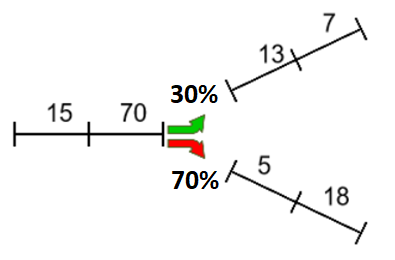
\includegraphics[width=10cm]{images/env_11_1570137518_procenty.png}
	\label{fig:env_11_case_0}
\end{figure}\noindent
\begin{itemize}
	\item Zatory są na odcinkach 0,1,2 i 5 (odpowiednio ilości pojazdów to 15,70,13,18). 
	\item Obecna faza świetlna to 0.
\end{itemize}
Najistotniejszym punktem macierzy sygnalizacji świetlnej jest $ S[1,2]=1 $, co odpowiada zielonemu światłu dla lewoskrętu. Cała macierz $ \textbf{S} $ to:
\def \ScaseZero {\begin{bmatrix}
		1 & 0 & 0 & 0 & 0 & 0 \\
		1 & 1 & 0 & 0 & 0 & 0 \\
		0 & 1 & 1 & 0 & 0 & 0 \\
		0 & 0 & 1 & 1 & 0 & 0 \\
		0 & 0 & 0 & 0 & 1 & 0 \\
		0 & 0 & 0 & 0 & 1 & 1 
\end{bmatrix}}
\def \AcaseZero {\begin{bmatrix}
		\frac{5}{15}  & 0             & 0             & 0 & 0 & 0 \\
		\frac{10}{15} & \frac{60}{70} & 0             & 0 & 0 & 0 \\
		0          	  & \frac{10}{70} & \frac{3}{13}  & 0 & 0 & 0 \\
		0             & 0             & \frac{10}{13} & 0 & 0 & 0 \\
		0             & 0             & 0             & 0 & 0 & 0 \\
		0             & 0             & 0             & 0 & 1 & 0 
\end{bmatrix}}

\[\textbf{S}= \ScaseZero \addtag \]
Macierz systemu to zatem:
\[\textbf{A}= \AcaseZero \addtag \]
\def \utMinusI{\begin{bmatrix} 
		7 \\ 0 \\ 0 \\ 0 \\ 0 \\ 0 
\end{bmatrix}}
\def \xtMinusI{\begin{bmatrix} 
		15 \\ 70 \\ 13 \\ 7 \\ 5 \\ 18	
\end{bmatrix}}
\def \xt{\begin{bmatrix} 
		12 \\ 70 \\ 13 \\ 10 \\ 0 \\ 5	
\end{bmatrix}} \noindent
Dla przykładu szczegółowo zostaną policzone wartości zerowej kolumny macierzy $\textbf{A}$, która dotyczy pojazdów wyjeżdżających z odcinka 0. Pozostałe wartości są liczone analogicznie.
\begin{itemize}
	\item Korzystając ze wzoru \ref{eq:manewr_zator_f10} ustalone zostaje $f(0,1)=\frac{10}{15}$. Jest to przypadek zatoru i jedynie 10 pojazdów z 15 przemieszcza się do następnego odcinka.
	\item Wartości $f(0,2),(0,3),(0,4),(0,5)$ są równe $0$, gdyż są to przypadki \ref{eq:manewr_not_existing_f10} nieistniejących manewrów.
	\item $A[0,0]=1-\delta(0)=1-f(0,1)-f(0,2)-f(0,3)-f(0,4)-f(0,5)=1- \frac{10}{15} -0-0-0-0= \frac{5}{15}$
\end{itemize}
Stan w momencie $t=1$ wyliczony z równania stanu jest następujący:
\[\textbf{x[1]}=\textbf{A[0]x[0]}=\AcaseZero \cdot \xtMinusI = \xt \]
Poniższy obraz przedstawia sytuację w środowisku w chwili t-1 oraz przepływ pojazdów, który miał miejsce między momentem $t-1$ a $t$.
\begin{figure}[H]
	\centering
	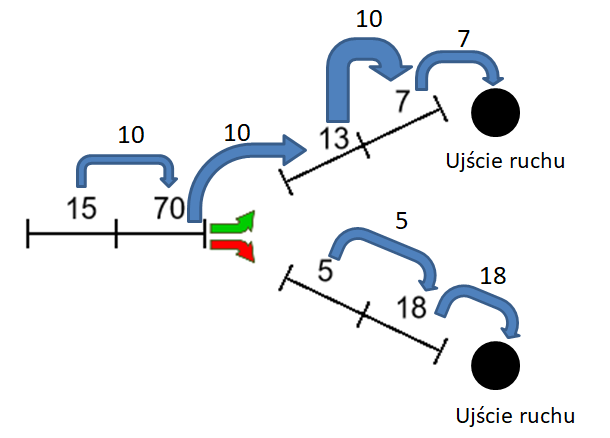
\includegraphics[width=10cm]{images/env_11_przeplyw_korek}
	\label{fig:env_11_case_0_przeplyw}
\end{figure}\noindent
W rezultacie w chwili t obecny jest następujący stan:
\begin{figure}[H]
	\centering
	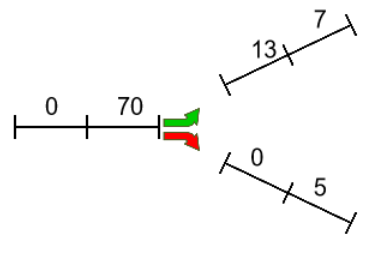
\includegraphics[width=10cm]{images/env_11_po_korku}
	\label{fig:env_11_case_0_po_przeplywie}
\end{figure}\noindent


\chapter {środowiska symulacyjne}
W tym rozdziale przedstawione zostaną środowiska symulacyjne. Głównym ich elementem jest sieć dróg. Podstawowe informacje na temat działania modelu sieci dróg i ruchu obowiązującego na nich zostały przedstawione w rozdziale \ref{chapter:model_sieci_drog}. Drugim elementem środowiska symulacyjnego są agenci. Są oni odpowiedzialni za dokonywanie decyzji związanych z sygnalizacją świetlną. 
\section{Srodowisko 1(11 na froncie)}
Elementy sieci dróg pierwszego środowiska były niejednokrotnie przedstawiane w rozdziale \myref{chapter:model_sieci_drog}, jednak dopiero teraz nastąpi przedstawienie pierwszego pełnego środowiska symulacyjnego. Na model sieci składają się 3 drogi - każda ma po 2 odcinki. Jest jedno skrzyżowanie na którym 75 procent pojazdów skręca w prawo, a pozostałe obierają kierunek w lewo.
	\begin{figure}[H]
	\centering
	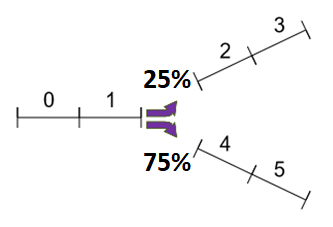
\includegraphics[width=10cm]{images/env_11_procenty}
	\label{fig:env_11}
	\caption{środowisko 11}
\end{figure}

\subsection{Sygnalizacje świetlne}	
\begin{figure}[H]
	\centering
	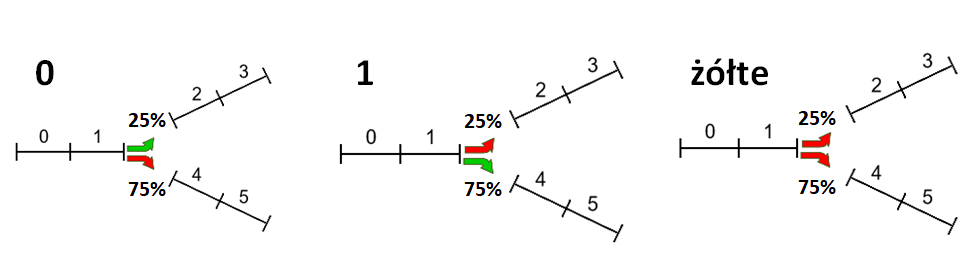
\includegraphics[width=17cm]{images/env_11_fazy_procenty}
	\label{fig:env_11_fazy}
	\caption{środowisko 11 - fazy świateł}
\end{figure}\noindent
Skrzyżowanie posiada 3 fazy świetlne przedstawione powyżej. Faza 0 umożliwia skręt w lewo (manewr [1,2]) z kolei faza 1 umożliwia skręt w prawo (manewr [1,4]). Faza żółte blokuje przejazd przez skrzyżowanie.

\subsection{Przestrzeń decyzyjna}
Przestrzeń decyzyjną oraz konsekwencje akcji podjętych przez agenta przedstawia poniższa tabela:

\begin{figure}[H]
	\centering
	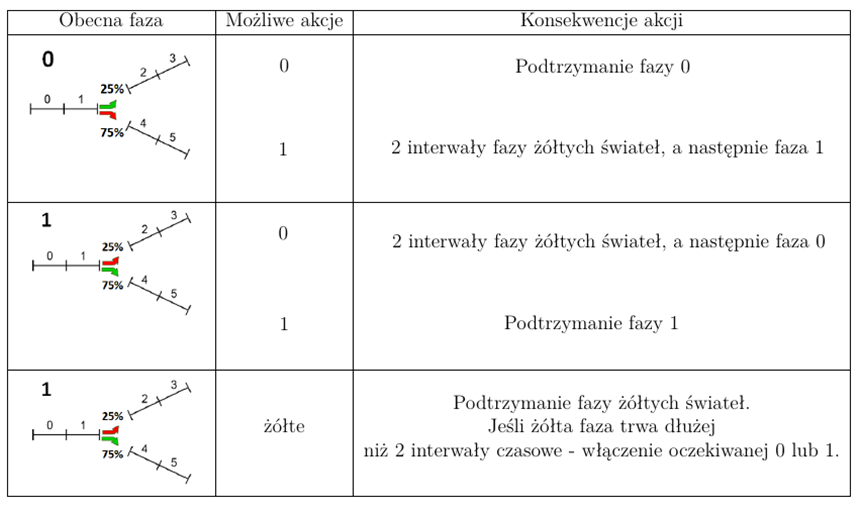
\includegraphics[width=17cm]{images/env_11_tabela_akcji}
	\label{fig:env_4_tabela_akcji}
\end{figure}
W przypadku zmiany fazy świetlnej następuje okres 2 interwałów żółtych świateł. Agent może także podtrzymać aktualną fazę świetlną.

\subsection{Zatory drogowe}
Wykorzystana w modelu zostanie funkcja zatoru przedstawiona w rozdziale \myref{subsec:zator_f10}, czyli:

\begin{numcases}{f(i,j)=}
\textbf{P}[i,j] & dla $ j=i+1 \wedge x[i]<10$ - przejazd bez zatoru \label{eq:manewr_bez_zatoru_f10} \\
\frac{10}{x[i]} & dla $ j=i+1  \wedge x[i] \geq 10$ - przejazd z zatorem \label{eq:manewr_zator_f10} \\
0 & dla pozostałych przypadków - manewr [i,j]
\end{numcases} \noindent


\section{Srodowisko 4}
\begin{figure}[H]
	\centering
	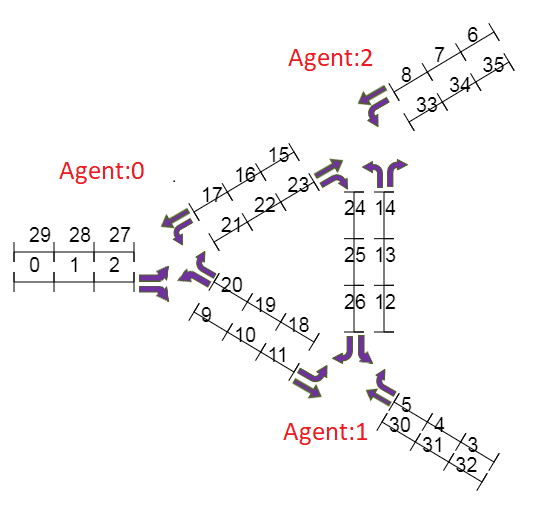
\includegraphics[width=10cm]{env_4_agenci}
	\label{fig:env_4_agenci}
	\caption{środowisko 4}
\end{figure}

środowisko posiada 12 jednokierunkowych dróg. Każda droga ma 3 odcinki co daje w sumie 36 odcinków (są numerowane od 0 co widać na rysunku \ref{fig:env_4_agenci}).
W sieci dróg znajdują się 3 skrzyżowania. Do każdego z nich jest przypisany agent, który odpowiada za sterowanie sygnalizacją świetlną.

Model ruchu:
Pojazdy w jednym interwale czasowym pokonują jeden odcinek. Na skrzyżowaniach w przypadku zielonego światła przejeżdża maksymalnie 10 pojazdów w jedną stronę.
Fazy świetlne: Każde skrzyżowanie posiada 4 fazy świetlne przedstawione poniżej. Fazy 0,1 i 2 są fazami, które posiadają pewne zielone światła. Agent podejmuje decyzję o zmianie tych faz. Zmiana ta nie jest natychmiastowa i następuje dopiero po 2 interwałach fazy żółtych 
świateł.

\begin{figure}[H]
	\centering
	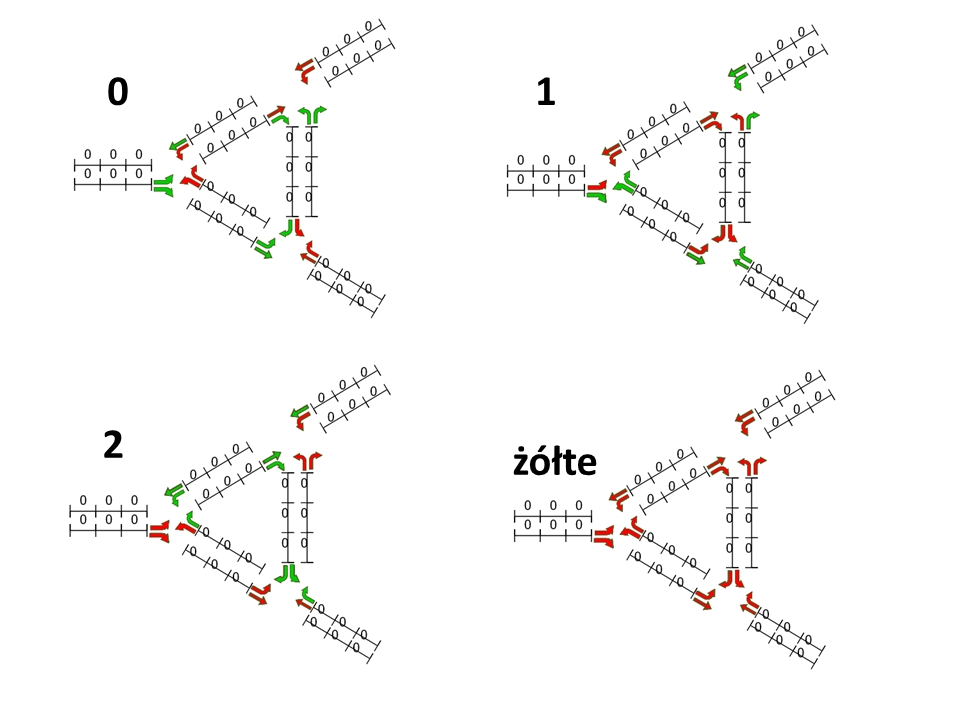
\includegraphics[width=14cm]{env_4_fazy}
	\label{fig:env_4_fazy}
	\caption{środowisko 4 - fazy świateł}
\end{figure}


Uczenie:
Każdy agent jako stan przyjmuje 10 elementową tablicę. 9 elementów to ilości pojazdów na odcinkach będących przed skrzyżowaniem przypisanym do agenta.
\chapter{Przegląd metod optymalizacyjnych}
\section{Kategorie uczenia maszynowego}
Uczenie maszynowe to dziedzina wchodząca w skład nauk zajmujących się sztuczną inteligencją. Samo uczenie w najprostszym kształcie może być rozumiane jako dobór parametrów na podstawie dostępnych danych. Uczenie maszynowe jest powszechnie dzielone na 3 kategorie nauki \cite{machineLearningClassification}.
\begin{enumerate}
	\item \textbf{Nadzorowane} \\
	Dane używane do uczenia nazywane są zbiorem treningowym. Każdy pojedynczy element zbioru treningowego ma informacje wejściowe oraz pewną pożądaną wartość wyjściową. W trakcie uczenia algorytm dopasowuje swoje parametry tak aby na podstawie danych wejściowych mógł przewidzieć wartość wyjściową. Przykładami uczenia nadzorowanego jest np. rozpoznawanie tekstu pisanego, detekcja obiektów na zdjęciach.
	\item \textbf{Nienadzorowane}
	Uczenie nienadzorowane różni się od nadzorowanego tym, że nie  są znane pożądane wartości wyjściowe. Celem nauki jest na podstawie podobieństw poszczególnych elementów zgrupowanie ich do odpowiednich klas. Przykładem uczenia nienadzorowanego może być np. klasyfikacja gatunków drzew na podstawie danych o ich wysokościach i szerokości korony drzew.
	\item \textbf{Wzmocnione}
	W środowisku uczenia ze wzmocnieniem istnieje agent, który jest odpowiedzialny za podejmowanie pewnych decyzji. Każda decyzja ma wpływ na stan środowiska, które zwraca agentowi nagrodę. Celem uczenia ze wzmocnieniem jest ustalenie strategii maksymalizującej skumulowaną wartość nagród.
\end{enumerate}
Ze wszystkich trzech kategorii uczenie ze wzmocnieniem odpowiada problemowi rozważanym w rozdziale Y. Szczegółowy opis uczenia ze wzmocnieniem zostanie przedstawiony w następnej sekcji.
\section{Uczenie ze wzmocnieniem}
Schemat uczenia ze wzmocnieniem składa się z następujących elementów:
\begin{enumerate}
	\item \textbf{Agent} jest odpowiedzialny za podejmowanie pewnych decyzji. Ma on wiedzę na temat obecnego stanu środowiska i otrzymuje w każdym kroku czasowym sygnał nagrody. Jego decyzje niebezpośrednio wpływają na stan środowiska.
	\item \textbf{Środowisko} jest przestrzenią posiadającą dynamiczny stan widoczny dla agenta. Chociaż to agent podejmuje akcje, to środowisko ma zdefiniowany model zmiany stanu. Model zmiany stanu może być stochastyczny oraz niewidoczny dla agenta. Oznacza to, że dwie te same akcje podjęte w tym samym stanie nie zawsze przyniosą identyczny następny stan. Innymi słowy agent nie może być stuprocentowo pewny rezultatów swoich akcji. Środowisko jest także nadawcą sygnału nagrody.
	\item \textbf{Strategia} definiuje sposób doboru akcji przez agenta w danej chwili. Jest to funkcja, która przyjmuje stan środowiska i zwraca akcje, która ma być przeprowadzona. 
	\item \textbf{Sygnał nagrody} definiuje cel problemu uczenia ze wzmocnieniem. W każdym kroku czasowym środowisko wysyła agentowi liczbę rzeczywistą, która jest nazywana nagrodą(reward). Wartości nagród są czynnikiem wpływającym na zmianę strategii, gdyż zadaniem agenta jest maksymalizacja nagród. Wartość nagród zatem definiuje, które zdarzenia są dobre, a które złe dla agenta. Biologicznym odpowiednikiem dodatniej nagrody jest przyjemność, a ujemnej - ból. 
	\item \textbf{Funkcja wartości} zwraca wartość stanu czyli oczekiwaną sumę nagród jakie agent osiągnie w przyszłości będąc aktualnie w tym stanie. 
\end{enumerate}
\begin{figure}[H]
	\centering
	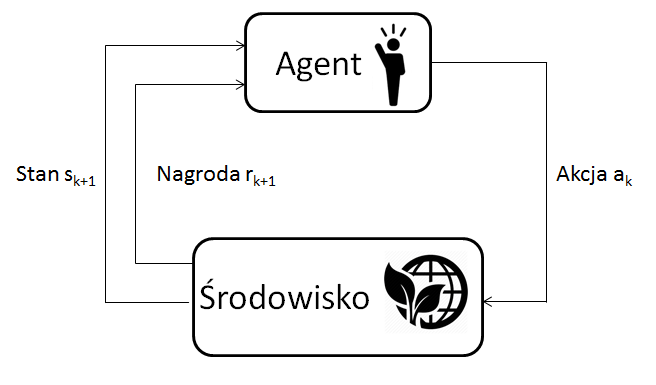
\includegraphics[width=14cm]{agent-srodowisko}
	\caption{Interakcje pomiędzy agentem a środowiskiem.}
	\label{fig:agent-srodowisko}
\end{figure}
\newpage
Algorytmy uczenia ze wzmocnieniem zazwyczaj stosuje się do rozwiązywania problemu procesu decyzyjnego Markowa. Sam \textbf{proces decyzyjny Markowa} jest zdefiniowany jako uporządkowana czwórka $(S,A,P_a,R_a)$, gdzie:
\begin{enumerate}
	\item $S$ to zbiór stanów
	\item $A$ to zbiór akcji. Notacją $A_s$ oznaczane są możliwe akcje dla stanu $s$.
	\item $P_a(s,s')=Pr(s_{t+1}=s'|s_t=s,a_t=a)$ to prawdopodobieństwo, że akcja $a$ wykonana w stanie $s$ w chwili $t$ doprowadzi do stanu $s'$ w chwili $t+1$.
	\item $R_a(s,s')$ to oczekiwana nagroda otrzymana w wyniku akcji podjętej w stanie $s$ prowadzącej do stanu $s'$.
\end{enumerate}

Problemem procesu decyzyjnego Markowa jest odnalezienie optymalnej strategii. Strategia określona jest jako funkcja $\pi(s)$ przyjmująca jako argument stan, a zwracająca podejmowaną akcję. Celem optymalizacji jest odnalezienie strategii maksymalizującej wartość:
\[
G=\sum_{k=0}^{K} \gamma^k R_{k} \addtag \label{eq:Markov_maximize}
\]
Chociaż strategii $\pi(s)$ nie ma we wzorcze \ref{eq:Markov_maximize}, to strategia wpływa na otrzymywane nagrody $R_{k}$ w każdej chwili $k$.\\
$\gamma \in (0,1]$ jest czynnikiem dyskontującym. Idea dyskontowania nagród zaczerpnięta jest z rachunku finansowego. Przykładowo wpływ na konto kapitału 1000 złotych po upływie roku czasu jest z pewnością bardziej wartościowy niż za 20 lat. Innymi słowy - pieniądze są liczone w czasie i tak samo należy postępować z nagrodami. Im wartość $\gamma$ jest bliższa 0 tym bardziej istotne są początkowe nagrody. Dla $\gamma=1$ wszystkie nagrody są równie istotne - bez względu na czas ich otrzymania.\\
Analogicznie do (\ref{eq:Markov_maximize}) jest ustalona funkcja wartości stanu. Jako wartość stanu $s$ określone jest:
\[
G_t=\sum_{k=t}^{K} \gamma^k R_{k}=R_{t}+\gamma R_{t+1}+\gamma^{2} R_{t+2}+...+\gamma^{K}R_K \addtag \label{eq:Markov_state_value_G}
\]
Zostanie przedstawiony teraz przykład obliczeniowy. Agent podejmuje decyzje na których podstawie otrzymuje ciąg  nagród $R_0=0, R_1=2,R_2=6,R_3=-1,R_4=2,R_5=1$. Czynnik dyskontujący $\gamma$ jest równy 0,9. Jaka jest wartość $G$ oraz $G_1,G_2,G_3,G_4,G_5$?\\
\begin{figure}[H]
	\centering
	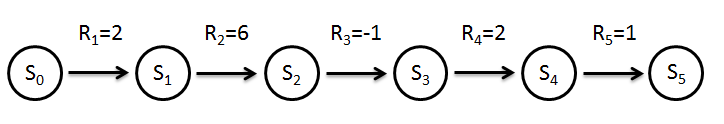
\includegraphics[width=14cm]{rewards-graph}
	\caption{Ciąg nagród i stanów.}
	\label{fig:agent-srodowisko}
\end{figure}\noindent
Najłatwiej obliczenia rozpocząć od $G_5$, ponieważ
\[G_{t}=R_{t}+\gamma G_{t+1} \label{eq:G_reccurential} \addtag \].\\
$G_5=R_5=1$.\\
$G_4=R_4+\gamma G_{5}=\;\;2+0,9\cdot 1=2,9$\\
$G_3=R_3+\gamma G_{4}=\!-1+0,9\cdot2.9=1,61$\\
$G_2=R_2+\gamma G_{3}=\;\;6+0,9\cdot1,61 \approx 7,45$\\
$G_1=R_1+\gamma G_{2}=\;\;2+0,9\cdot 7,45 \approx 8,70$\\
$G\;\,=R_0+\gamma G_{1}=\;\;0+0,9\cdot 8,70 \approx 7,83$\\

\section{Programowanie dynamiczne}
Termin programowania dynamicznego odnosi się do algorytmów wyliczających optymalne strategie procesu decyzyjnego Markowa w przypadku posiadanej całkowitej wiedzy na temat modelu środowiska\cite{reinforcementBook}. Środowisko nie musi być w pełni deterministyczne tzn. nie za każdym razem akcja przeprowadzana ze stanu $s_k$ musi w efekcie doprowadzić do tego samego stanu $s_{k+1}$. Jednak w takim przypadku musi być znany rozkład prawdopodobieństwa przydzielania nowego stanu na podstawie poprzedniego i właśnie podjętej przez agenta akcji. Dodatkowo wymagana jest możliwość ustalenia dowolnego stanu w trakcie uczenia. \\ Początkowa strategia $\pi(s)$ jest dowolna, najczęściej losowa.
Przedstawiony algorytm jest podzielony na 2 części. Część predykcji(prediction) oraz kontroli (control). 
\\\textbf{Proces predykcji} ma za zadanie ustalenie wartości stanów na podstawie ustalonej strategii. Jej algorytm jest następujący:
\begin{enumerate}
	\item{Przyjmij daną z góry $\pi$ jako strategię podejmowania akcji}
	\item{Zainicjuj tablicę wartości stanów $V(s)$. Dla wszystkich możliwych stanów $s \in S$ przyjmij wartość $0$.}
	\item{$\Delta=0$}
	\item{Dla każdego $s \in S$:}
	\begin{enumerate}
		\item $v=V(s)$
		\item $V(s)=\sum_{s'}Pr(s'|s,\pi(s))[r+\gamma V(s')]$
		\item $\Delta = max(\Delta,|v-V(s)|)$
	\end{enumerate}
	\item Jeśli $\Delta< \theta$ to wróć do 3
	\item Zwróć $V(s)$ jako tablicę wartości stanów $V_{\pi}(s)$ dla strategii $\pi$.
\end{enumerate}
Parametr $\theta \geq 0$ definiuje w kroku 5. moment stopu. \\
Wartość $Pr(s',s,\pi(s))$ to prawdopodobieństwo, że akcja $\pi(s)$ podjęta w stanie $s$ doprowadzi do stanu $s'$. Z kolei $r$ jest właśnie otrzymaną nagrodą.
\\ Algorytm \textbf{kontroli} ma za zadanie odnaleźć bardziej optymalną strategię niż dotychczas. Jako argument przyjmuje on wyliczoną właśnie tablicę wartości stanów $V_{\pi}(s)$. Wprowadzona zostaje macierz $Q_{\pi}(s,a)$. Jest ona zdefiniowana następująco:
\begin{equation}
\begin{split}
Q_{\pi}(s,a) &= E[R_{t+1}+\gamma v_{\pi}(S_{t+1}) | S_t=s, A_t=a]  \\
&= \sum_{s'}Pr(s'|s,a)[r+\gamma V_{pi}(s')] 
\end{split}
\end{equation}
Oczywistym minusem tego algorytmu jest konieczność przeiterowania wszystkich stanów. W przypadku gdy stanów jest bardzo dużo algorytm staje się nieopłacalny.
Macierz przedstawia wartość akcji $a$ podjętej w stanie $s$. Algorytm kontroli jest następujący:
\begin{enumerate}
	\item{Przyjmij wyliczoną przez algorytm predykcji macierz wartości stanów $V_{\pi}(s)$}
	\item{Zainicjuj tablicę wartości stanów $V(s)$. Dla wszystkich możliwych stanów $s \in S$ przyjmij wartość $0$.}
	\item{$policy\_stable=false$}
	\item{Dla każdego $s \in S$:}
	\begin{enumerate}
		\item $old\_action=\pi(s)$
		\item $\pi(s)=argmax_{a\in A_s} \sum_{s'}Pr(s'|s,a)[r+\gamma V(s')]$
		\item Jeśli $old\_action \neq \pi(s)$ to $policy\_stable = true$
	\end{enumerate}
	\item Jeśli $policy\_stable=true$ to zwróć strategię $\pi(s)$.
\end{enumerate}
\section{Metoda Monte Carlo On-Policy}
Metody Monte Carlo są szeroką klasą algorytmów, których wyniki oparte są o losowe próbkowanie. Nie potrzebują one żadnej wiedzy na temat środowiska - akceptowalne są zarówno środowiska deterministyczne jak i stochastyczne. Algorytmy Monte Carlo uczenia ze wzmocnieniem są dzielone na dwie kategorie - On-Policy oraz Off-policy. W pracy zostanie przedstawiona metoda on-policy, która różni się od off-policy jedynie sposobem doboru momentu eksploracji. Metoda on-policy zakłada, iż ustalana jest pewna liczba $\epsilon$ bliska zeru. Określa ona prawdopodobieństwo kroku eksploracji, czyli wyboru losowej akcji. Pozostałe akcje są wybierane w sposób zachłanny, czyli podejmowana jest najbardziej wartościowa dostępna akcja. Algorytm przedstawiony jest poniższym pseudokodem.
\begin{enumerate}
	\item Zainicjuj słowniki:
	\begin{enumerate}
		\item $Q(s,a)$ - Wartość określa opłacalność wyboru akcji a w stanie s
		\item $Returns(s,a)$ - Wartość słownika to tablica wartości $G$ wyliczonych na podstawie wzoru (\ref{eq:Markov_state_value_G}).
		\item $\pi(s)$ - Określa jaka akcja ma zostać podjęta dla stanu s. Początkowo wszystkie akcje są wybrane losowo.
	\end{enumerate}
	\item Zasymuluj pełny epizod wedle strategii $\pi$
	\item Zoptymalizuj strategię $\pi$ - dla każdej pary (s,a) - stanu i akcji, które pojawiły się w epizodzie
	\begin{enumerate}
		\item Wylicz $G$ rekurencyjnie wedle wzoru (\ref{eq:G_reccurential}) t.j. $G_{t}=R_{t}+\gamma G_{t+1}$. *
		\item Do tablicy Returns(s,a) dodaj wartość $G$
		\item $Q(s,a)=avg(Returns(s,a))$
		\item $\pi(s)=a^*$. Gdzie $a^*$ to taka akcja, że $Q(s,a^*)\geq Q(s,a)$ dla każdego $a 
		\in A$. Jeśli został jednak wylosowany krok ekspolarcji, wtedy $\pi(s)$ jest losowo wybraną akcją $a \in A$.
	\end{enumerate}
\end{enumerate}
* - Rozsądnym jest iterowanie w 3 kroku w kolejności odwrotnej do chronologicznej, gdyż ułatwia wykorzystanie wzoru (\ref{eq:G_reccurential})
\\ Warto zauważyć następujące zalety metody Monte Carlo, których nie zapewniał algorytm programowania dynamicznego:
\begin{enumerate}
	\item Brak potrzeby wiedzy na tematu modelu
	\item Nie wymaga często nierealnego założenia, iż stan środowiska może zostać sztywno ustalony przez programistę. Wymagana jest jedynie możliwość przeprowadznia pełnych epizodów, co jest nieporównywalnie słabszym założeniem.
	\item Dobre skalowanie dla dużej przestrzeni stanu. Więcej czasu treningowego jest poświęcane dla stanów, które są często odwiedzane. Z kolei te, które nie pojawiają się prawie wcale - nie marnują dużo czasu w procesie nauki.
\end{enumerate}









\bibliography{refs}
\end{document}
